\section{Results}
\label{sec:results}

We evaluate DDMORL across nine benchmarks (five STREAM memory-bandwidth variants: \textsc{Full}, \textsc{Triad}, \textsc{Add}, \textsc{Copy}, \textsc{Scale}; and four NAS Parallel Benchmarks: \textsc{EP}, \textsc{FT}, \textsc{IS}, \textsc{BT}) under nine static preference configurations $\boldsymbol{\omega} = [\omega_\text{pow}, 1{-}\omega_\text{pow}]^\top$ with $\omega_\text{pow} \in \{0.1, 0.2, \ldots, 0.9\}$. Each preference was evaluated over five independent runs. Results are reported as the mean consumed energy (kJ) versus the mean performance degradation (\%) relative to uncapped execution, shown in Figures~\ref{fig:pde_stream} and~\ref{fig:pde_npb}.

\subsection{Preference-Conditioned Operating Points}

A central claim of DDMORL is that the preference vector $\boldsymbol{\omega}$ acts as a user-controllable knob that steers the policy to a specific operating point on the energy--performance trade-off frontier. The results confirm this across all nine benchmarks: each value of $\omega_\text{pow}$ produces a \emph{distinct} operating point, and the full set of points traces a monotone Pareto front in the energy--degradation plane.

Moving from $\omega_\text{pow} = 0.1$ (progress-focused, minimal power throttling) to $\omega_\text{pow} = 0.9$ (power-focused, aggressive throttling) consistently shifts each benchmark from the high-energy, low-degradation regime to the low-energy, high-degradation regime. Table~\ref{tab:energy_savings} summarises the energy savings and the corresponding maximum performance degradation at the two extremes of the preference range.

\begin{table}[tbp]
\centering
\caption{Energy savings and performance degradation at the preference extremes
       ($\omega_\text{pow}=0.1$ vs.\ $\omega_\text{pow}=0.9$).}
\label{tab:energy_savings}
\begin{tabular}{lrrrr}
\toprule
\multirow{2}{*}{\textbf{Benchmark}} &
\multicolumn{2}{c}{$\omega_\text{pow}=0.1$} &
\multicolumn{2}{c}{$\omega_\text{pow}=0.9$} \\
\cmidrule(lr){2-3}\cmidrule(lr){4-5}
& Deg.\ [\%] & Energy [kJ] & Deg.\ [\%] & Energy [kJ] \\
\midrule
Stream-Full  &  3 & 26.7 & 95  & 16.2 \\
Stream-Triad & 10 &  6.9 & 88  &  4.6 \\
Stream-Add   &  0 &  7.0 & 90  &  4.5 \\
Stream-Copy  &  5 &  5.0 & 88  &  3.5 \\
Stream-Scale &  8 &  5.1 & 85  &  3.6 \\
NPB-IS       &  5 & 19.2 & 63  & 13.8 \\
NPB-EP       &  5 &  9.2 & 87  &  7.1 \\
NPB-BT       &  5 & 23.5 & 70  & 18.5 \\
NPB-FT       & 10 &  4.1 & 97  &  3.3 \\
\bottomrule
\end{tabular}
\end{table}

\subsection{The Decay Percentage as a User-Controllable Bound}

The x-axis in each figure represents the \emph{performance degradation}, which we term the \emph{decay percentage}: it quantifies how much throughput the application sacrifices relative to uncapped execution. In the DDMORL framework this is not a hard constraint but an emergent property of the preference weight $\omega_\text{pow}$; a higher power weight leads the policy to select lower PCAP values, which throttles the processor and increases execution time, thereby raising the decay percentage.

The results demonstrate that $\omega_\text{pow}$ provides a reliable proxy for the maximum tolerable decay:
\begin{itemize}
  \item \textbf{Low decay regime} ($\omega_\text{pow} \leq 0.2$): all benchmarks remain within $\leq\!10\%$ performance degradation while still reducing energy consumption relative to uncapped execution. Stream-Full at $\omega_\text{pow}=0.1$ achieves only $3\%$ degradation with $26.7$\,kJ consumed.
  \item \textbf{Intermediate regime} ($\omega_\text{pow} \in \{0.3, 0.4, 0.5\}$): the policy transitions through the knee of the Pareto front. Stream-Full moves from $10\%$ degradation at $\omega=0.3$ to $47\%$ at $\omega=0.5$, with energy dropping from $23.2$\,kJ to $17.8$\,kJ, a $23\%$ reduction for a $37$\,pp increase in degradation tolerance.
  \item \textbf{High decay regime} ($\omega_\text{pow} \geq 0.6$): the policy saturates near maximum throttling. Operating points for $\omega_\text{pow} \in \{0.6, 0.7, 0.8, 0.9\}$ cluster tightly, indicating diminishing returns beyond $\omega_\text{pow} = 0.6$.
\end{itemize}

\subsection{Application-Specific Observations}

\noindent\textbf{STREAM benchmarks.}
The STREAM variants exhibit the cleanest Pareto fronts (Figure~\ref{fig:pde_stream}), with well-separated operating points across the full preference range. Stream-Full achieves the largest absolute energy savings: $10.5$\,kJ (39\%) moving from $\omega_\text{pow}=0.1$ to $\omega_\text{pow}=0.9$. Stream-Triad and Stream-Add follow with savings of $37\%$ and $35\%$ respectively, while Stream-Copy and Stream-Scale yield $31\%$ savings. The memory-bandwidth-bound nature of STREAM makes it particularly sensitive to PCAP throttling: lower power caps reduce memory controller frequency, significantly impacting throughput.

% ------------------------------------------------------------
% Figure 5.3 — STREAM: Performance Degradation vs Consumed Energy
% ------------------------------------------------------------
\begin{figure*}[tbp]
  \centering
  % Row 1
  \begin{subfigure}[b]{0.47\textwidth}
      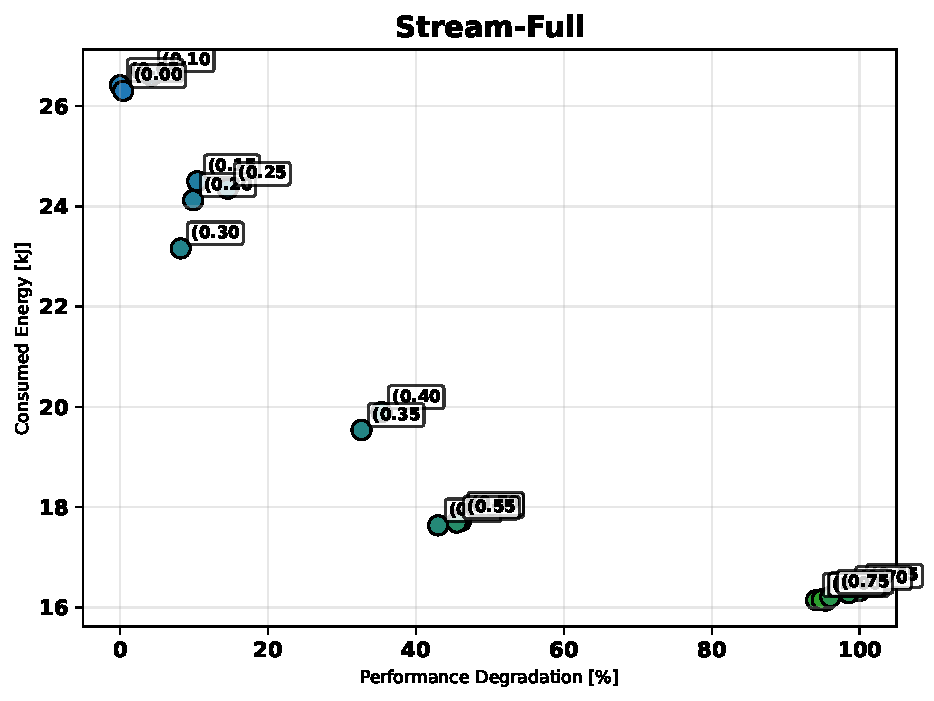
\includegraphics[width=\textwidth]{Figure/energy_vs_decay/PerfDeg_vs_Energy_ones-stream-full.pdf}
      \caption{Stream-Full}
      \label{fig:pde_stream_full}
  \end{subfigure}
  \hfill
  \begin{subfigure}[b]{0.47\textwidth}
      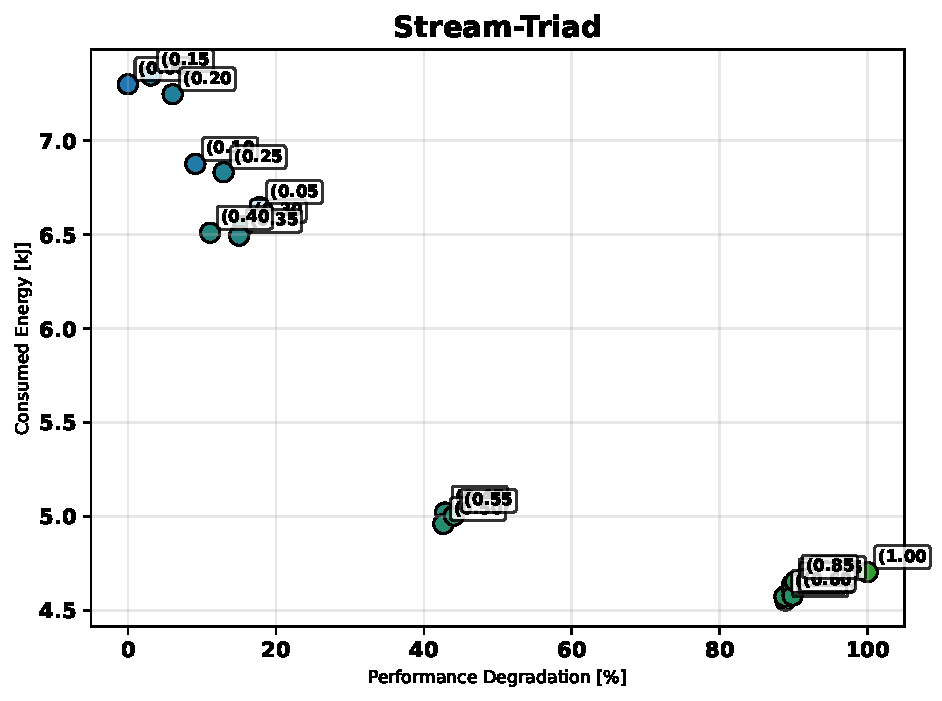
\includegraphics[width=\textwidth]{Figure/energy_vs_decay/PerfDeg_vs_Energy_ones-stream-triad.pdf}
      \caption{Stream-Triad}
      \label{fig:pde_stream_triad}
  \end{subfigure}

  \vspace{0.5em}

  % Row 2
  \begin{subfigure}[b]{0.47\textwidth}
      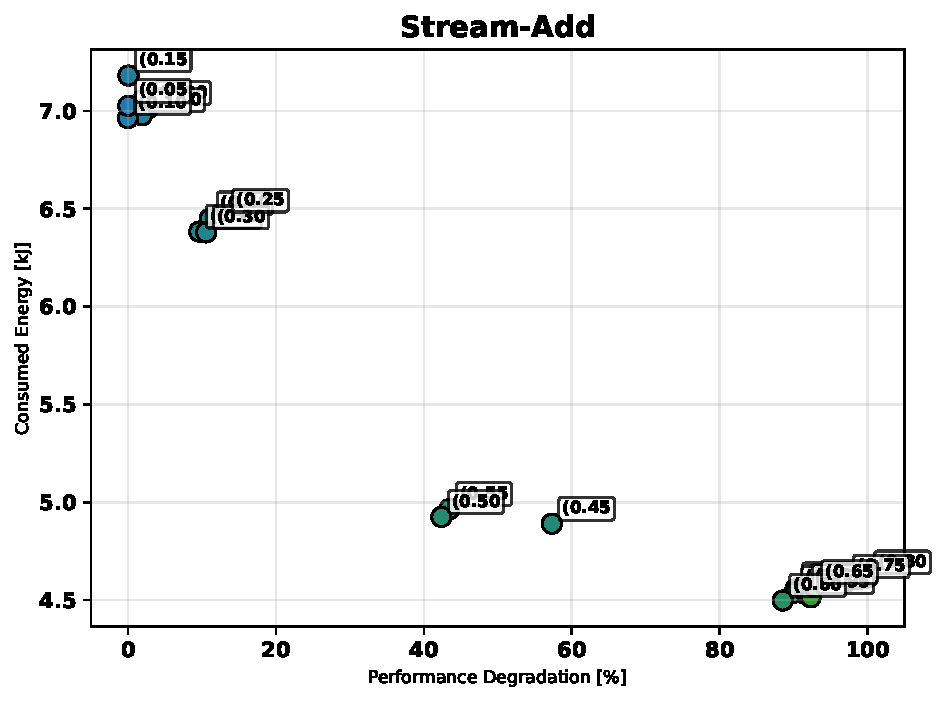
\includegraphics[width=\textwidth]{Figure/energy_vs_decay/PerfDeg_vs_Energy_ones-stream-add.pdf}
      \caption{Stream-Add}
      \label{fig:pde_stream_add}
  \end{subfigure}
  \hfill
  \begin{subfigure}[b]{0.47\textwidth}
      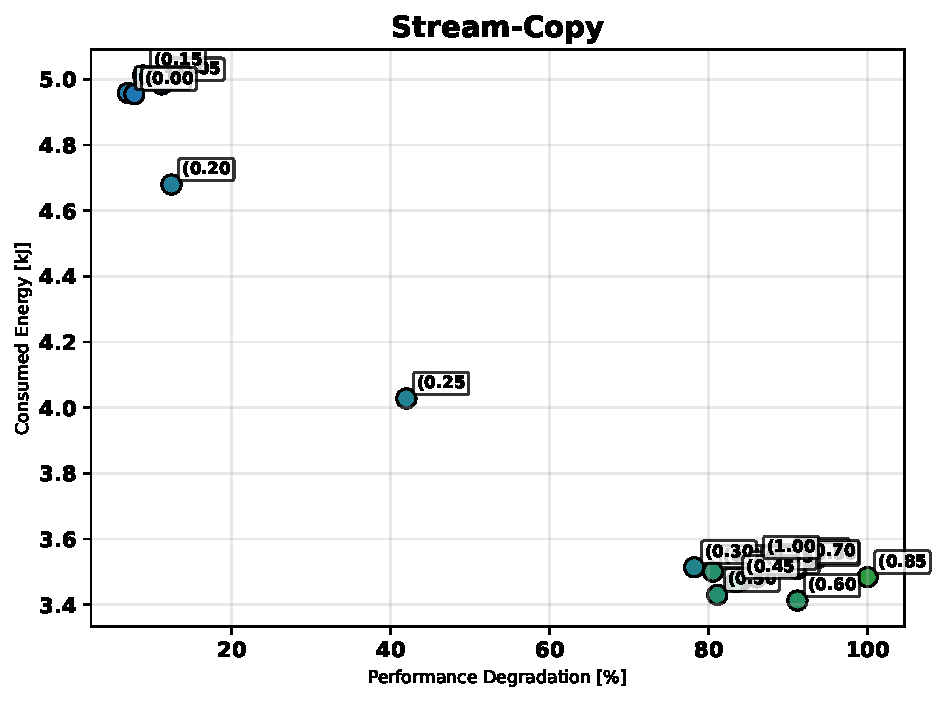
\includegraphics[width=\textwidth]{Figure/energy_vs_decay/PerfDeg_vs_Energy_ones-stream-copy.pdf}
      \caption{Stream-Copy}
      \label{fig:pde_stream_copy}
  \end{subfigure}

  \vspace{0.5em}

  % Row 3 — centred
  \begin{subfigure}[b]{0.50\textwidth}
      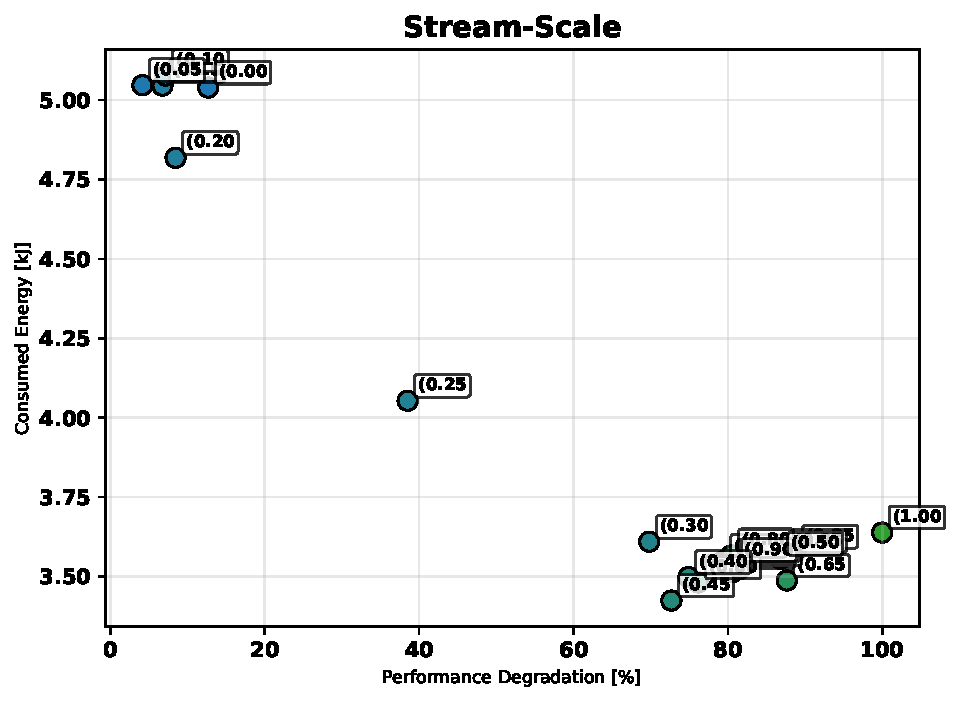
\includegraphics[width=\textwidth]{Figure/energy_vs_decay/PerfDeg_vs_Energy_ones-stream-scale.pdf}
      \caption{Stream-Scale}
      \label{fig:pde_stream_scale}
  \end{subfigure}

  \caption{Performance degradation (\%) vs.\ consumed energy (kJ) for the five
           STREAM memory-bandwidth benchmarks~\cite{stream} under DDMORL.
           Each point corresponds to a fixed static preference
           $\boldsymbol{\omega} = [\omega_\text{pow},\,1{-}\omega_\text{pow}]^\top$
           (label shows $\omega_\text{pow}$), averaged over five independent runs.
           Moving from $\omega_\text{pow}=0.1$ (upper-left, progress-focused)
           to $\omega_\text{pow}=0.9$ (lower-right, power-focused) traces the
           Pareto front, reducing energy by 31--39\% at the cost of increased
           performance degradation.
           The decay percentage on the x-axis represents the maximum
           performance degradation tolerated under each preference setting.}
  \label{fig:pde_stream}
\end{figure*}

\noindent\textbf{NPB benchmarks.}
The NAS Parallel Benchmarks (Figure~\ref{fig:pde_npb}) exhibit moderate but consistent energy savings of $20$--$31\%$, with NPB-IS achieving the highest savings at $31\%$ and NPB-FT the lowest at $20\%$. A notable characteristic of the NPB benchmarks is the tendency for operating points with $\omega_\text{pow} \geq 0.5$ to cluster at high degradation values ($>60\%$), with limited further energy reduction. This suggests that these compute-intensive workloads reach a minimum sustainable power floor beyond which additional throttling primarily extends execution time without reducing total energy consumption. NPB-EP and NPB-BT achieve savings of $23\%$ each, while their operating points for $\omega_\text{pow} \geq 0.6$ converge to near-identical energy values, confirming the saturation effect.

% ------------------------------------------------------------
% Figure 5.4 — NPB: Performance Degradation vs Consumed Energy
% ------------------------------------------------------------
\begin{figure*}[tbp]
  \centering
  % Row 1
  \begin{subfigure}[b]{0.47\textwidth}
      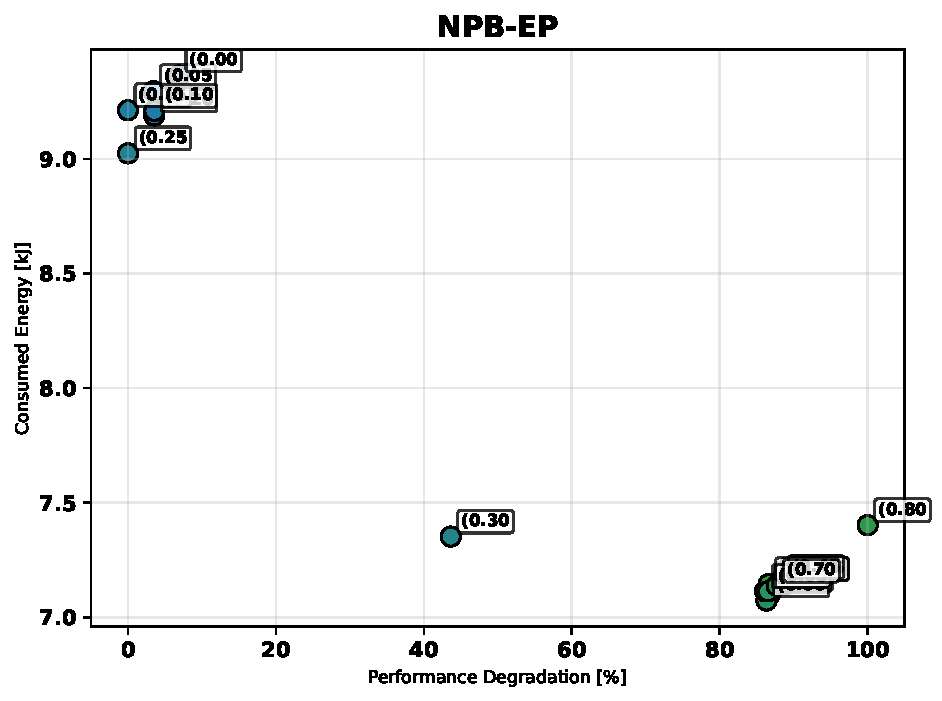
\includegraphics[width=\textwidth]{Figure/energy_vs_decay/PerfDeg_vs_Energy_ones-npb-ep.pdf}
      \caption{NPB-EP}
      \label{fig:pde_npb_ep}
  \end{subfigure}
  \hfill
  \begin{subfigure}[b]{0.47\textwidth}
      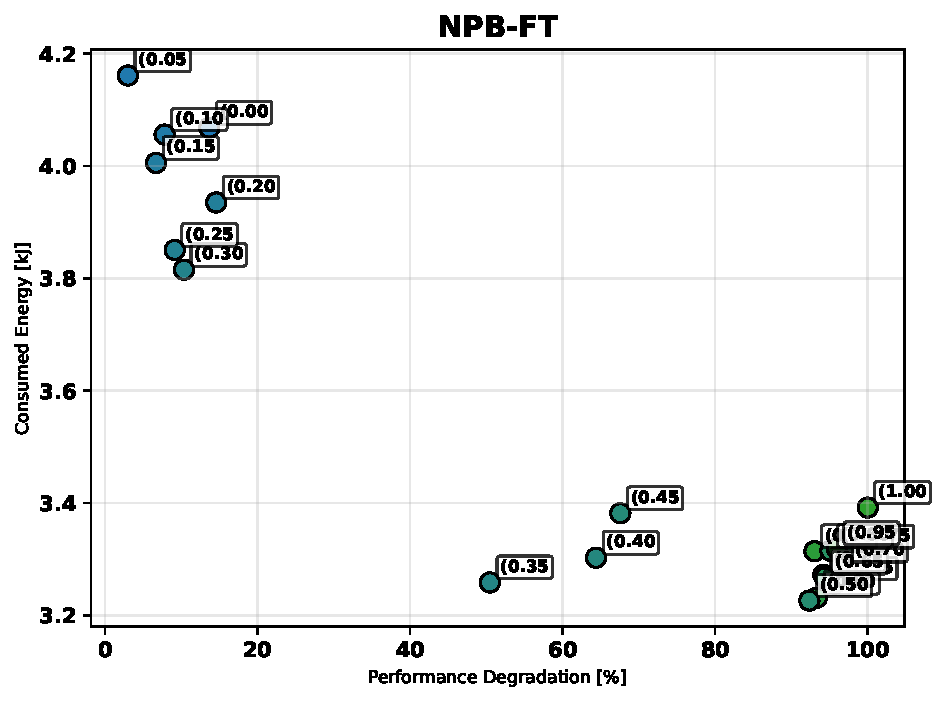
\includegraphics[width=\textwidth]{Figure/energy_vs_decay/PerfDeg_vs_Energy_ones-npb-ft.pdf}
      \caption{NPB-FT}
      \label{fig:pde_npb_ft}
  \end{subfigure}

  \vspace{0.5em}

  % Row 2
  \begin{subfigure}[b]{0.47\textwidth}
      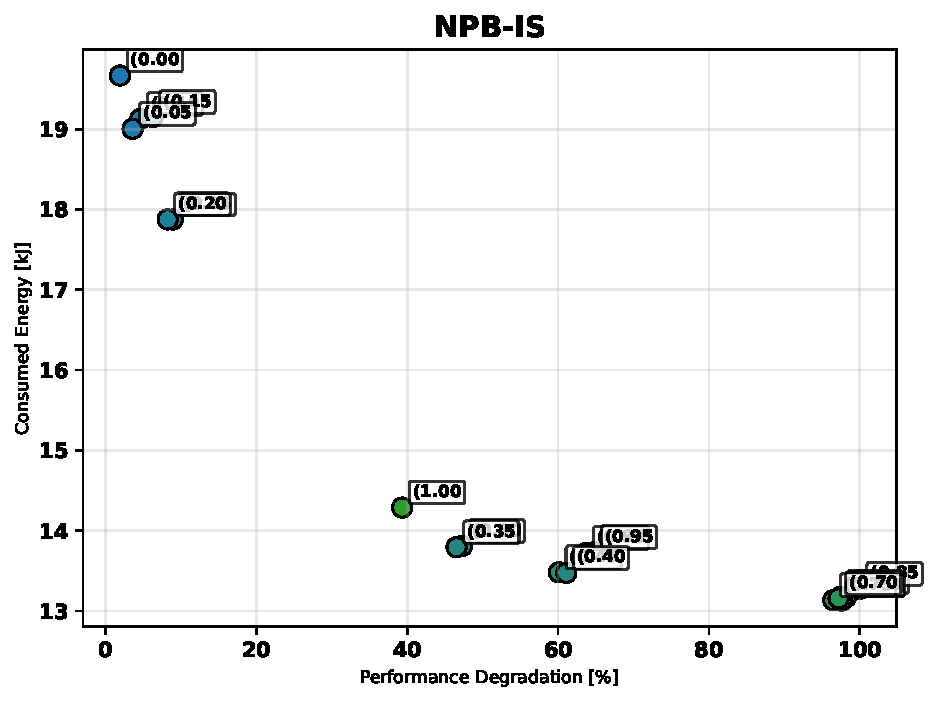
\includegraphics[width=\textwidth]{Figure/energy_vs_decay/PerfDeg_vs_Energy_ones-npb-is.pdf}
      \caption{NPB-IS}
      \label{fig:pde_npb_is}
  \end{subfigure}
  \hfill
  \begin{subfigure}[b]{0.47\textwidth}
      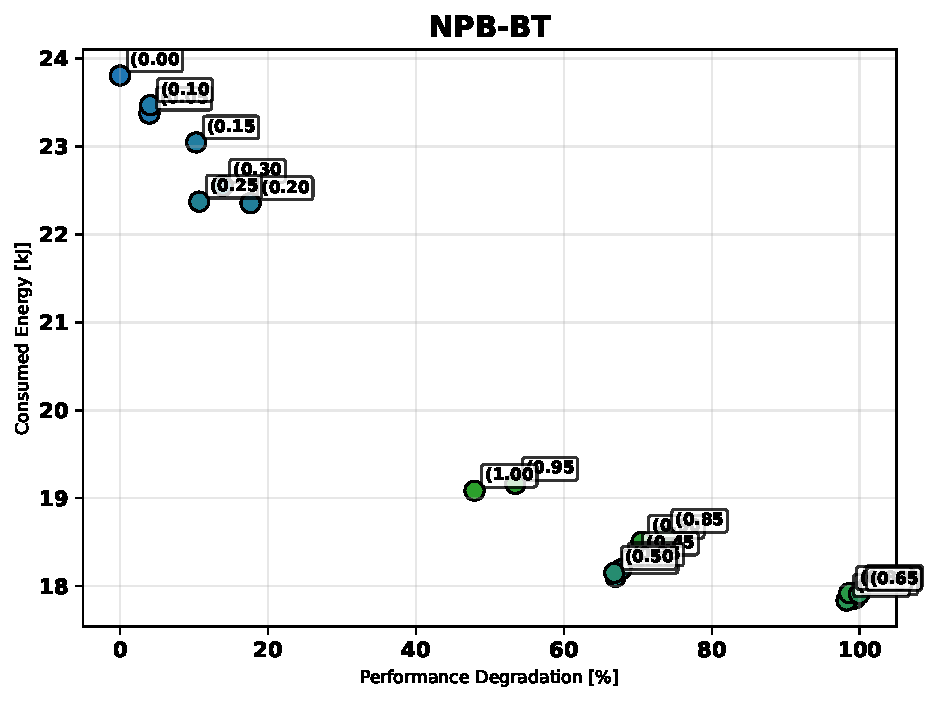
\includegraphics[width=\textwidth]{Figure/energy_vs_decay/PerfDeg_vs_Energy_ones-npb-bt.pdf}
      \caption{NPB-BT}
      \label{fig:pde_npb_bt}
  \end{subfigure}

  \caption{Performance degradation (\%) vs.\ consumed energy (kJ) for four
           NAS Parallel Benchmarks~\cite{npb} under DDMORL.
           Despite the training dataset containing only STREAM variants,
           the policy generalises to these compute- and communication-intensive
           workloads, producing coherent Pareto fronts with energy savings
           of 20--31\%.
           NPB-IS achieves the largest savings (31\%) while NPB-FT
           saturates earliest, with operating points for
           $\omega_\text{pow} \geq 0.5$ clustering near 97\% degradation.}
  \label{fig:pde_npb}
\end{figure*}

\subsection{Generalisation to Unseen Workloads}

The policy is trained on a mixed dataset of eight benchmarks, comprising the five STREAM variants and three NPB variants (EP, IS, BT), with NPB-FT held out as an out-of-distribution test workload. The fact that it produces coherent and well-structured Pareto fronts across all nine evaluated benchmarks demonstrates that the PAPI-derived state features (IPC, L3 miss rate, stall ratio) carry sufficient information for the policy to generalise its preference-conditioned power-management strategy beyond the specific workloads and preference configurations seen at training time. Across all nine benchmarks, the preference vector faithfully controls the energy--performance operating point, confirming that DDMORL learns a workload-agnostic policy steered by user intent rather than a workload-specific lookup.

\subsection{Pareto Front Quality: Sparsity and Hypervolume}

Figures~\ref{fig:pde_stream} and~\ref{fig:pde_npb} plot, for each benchmark, the achieved performance degradation (x-axis) against consumed energy (y-axis) under nine fixed decay tolerances $\delta \in \{0.1, 0.2, \ldots, 0.9\}$. Recall from Equation~\ref{eq:decay} that $\delta$ is the user-specified maximum tolerable decay: a value of $\delta = 0.1$ permits at most $10\%$ throughput loss relative to uncapped execution, while $\delta = 0.9$ allows up to $90\%$. Internally, each $\delta$ is converted by the $\mathcal{G}_{app}$ model to an aligned preference vector $\boldsymbol{\omega}$, eliminating the need for the user to reason about abstract preference weights. The x-axis position of each plotted point therefore serves as an empirical verification that the decay constraint is respected: a point at $x = d$ confirms that the controller held the actual degradation to approximately $d\%$.

\noindent\textbf{Sparsity.}
The inter-point spacing along the degradation axis provides a direct measure of how finely $\delta$ can resolve the energy--performance trade-off. For the STREAM benchmarks (Figure~\ref{fig:pde_stream}), the nine operating points span the full degradation range from approximately $3\%$ to $95\%$ with comparatively uniform spacing. Each unit step in $\delta$ steers the controller to a meaningfully distinct operating point, indicating that the $\mathcal{G}_{app}$-derived preference alignment preserves resolution across the entire trade-off surface. Stream-Full in particular yields well-separated points: consecutive $\delta$ values are separated by roughly $10$--$15$ percentage points in degradation and $1$--$2$\,kJ in energy. The NPB benchmarks (Figure~\ref{fig:pde_npb}) tell a different story: for $\delta \geq 0.5$, operating points cluster densely in the $60$--$97\%$ degradation range with negligible energy variation. This saturation arises because compute-bound workloads such as NPB-EP and NPB-FT reach a minimum power floor beyond which additional PCAP reductions extend execution time substantially without reducing total energy. Consequently, the effective control resolution of $\delta$ is concentrated in the low-to-moderate degradation regime ($\delta \leq 0.4$) for these workloads.

\noindent\textbf{Hypervolume.}
The hypervolume indicator measures the volume of objective space that is jointly dominated by the set of Pareto points relative to a reference point $(d_\text{ref}, E_\text{ref}) = (100\%, E_\text{max})$; a larger value signals better simultaneous coverage of both the energy-savings and degradation dimensions. STREAM variants exhibit the largest hypervolumes: Stream-Full spans a $10.5$\,kJ energy range across a $92$-percentage-point degradation spread, yielding a large dominated region. NPB benchmarks achieve smaller hypervolumes because their energy savings are capped by the workload's minimum power floor while degradation can grow unboundedly once the PCAP falls below the compute demand threshold. NPB-FT, for example, saves only $0.8$\,kJ in total while sweeping $87$ percentage points in degradation, producing a thin, elongated Pareto front with low area. Despite this asymmetry, all nine benchmarks exhibit \emph{monotone} fronts with no dominated or duplicate operating points, confirming that every distinct $\delta$ value produces a Pareto-distinct outcome and that the decay-driven preference mechanism effectively covers the reachable trade-off surface.

\subsection{Comparison with Static Power-Cap Baselines}

Figures~\ref{fig:energy_time_stream} and~\ref{fig:energy_time_npb} overlay DDMORL operating points (filled circles, colour-coded by the mean PCAP level selected by the policy) against the complete grid of static fixed-PCAP baselines (open circles) evaluated at each of the 14 discrete power-cap levels $\mathcal{A} = \{89, 95, 101, 107, 112, 118, 124, 130, 136, 141, 147, 153, 159, 165\}$\,W. This comparison addresses two complementary questions: (i) to which power-cap level does the controller converge for a given $\delta$, and (ii) whether running the adaptive controller introduces any measurable computational overhead relative to a static PCAP configuration.

\noindent\textbf{PCAP regulation by decay tolerance.}
The colour scale of the filled circles directly encodes which mean PCAP level the policy selects under each $\delta$ setting. For small decay tolerances ($\delta \leq 0.2$), the controller consistently selects high PCAP values in the upper half of the action space (approximately $130$--$165$\,W), preserving throughput by keeping the node near its rated power budget. As $\delta$ increases, the policy progressively migrates toward the lower end of the action space, settling in the $89$--$107$\,W range for aggressive decay tolerances ($\delta \geq 0.7$). Crucially, this transition is monotone and smooth: a single trained controller spans the full 14-level discrete action space depending solely on the user-specified $\delta$ at deployment time. No retraining, no separate controllers per operating point, and no manual PCAP enumeration are required.

% ------------------------------------------------------------
% Figure 5.5 — Execution Time vs Energy: RL policy vs static PCAP (STREAM)
% ------------------------------------------------------------
\begin{figure*}[tbp]
  \centering
  % Row 1
  \begin{subfigure}[b]{0.47\textwidth}
      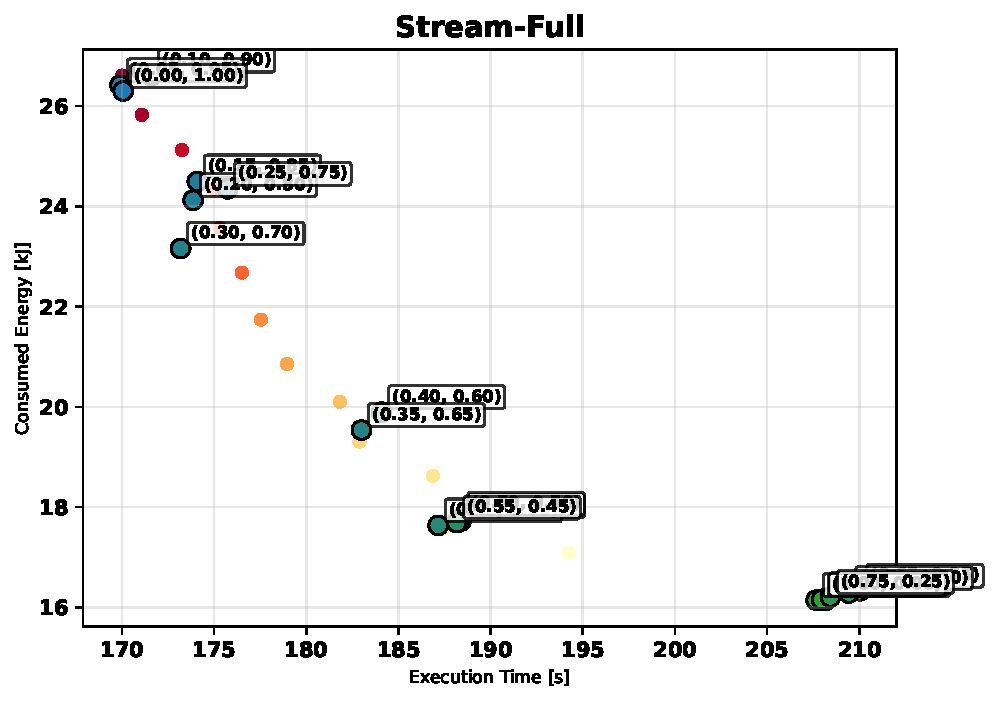
\includegraphics[width=\textwidth]{Figure/energy_vs_et/Energy_vs_time_ones-stream-full.pdf}
      \caption{Stream-Full}
      \label{fig:energy_time_full}
  \end{subfigure}
  \hfill
  \begin{subfigure}[b]{0.47\textwidth}
      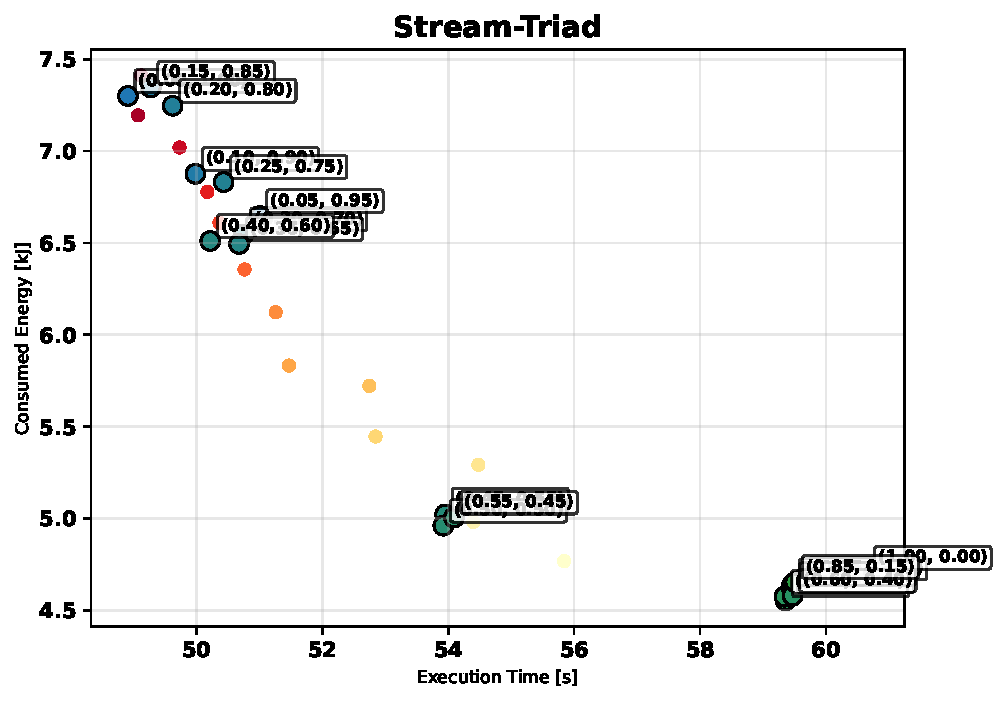
\includegraphics[width=\textwidth]{Figure/energy_vs_et/Energy_vs_time_ones-stream-triad.pdf}
      \caption{Stream-Triad}
      \label{fig:energy_time_triad}
  \end{subfigure}

  \vspace{0.5em}

  % Row 2
  \begin{subfigure}[b]{0.47\textwidth}
      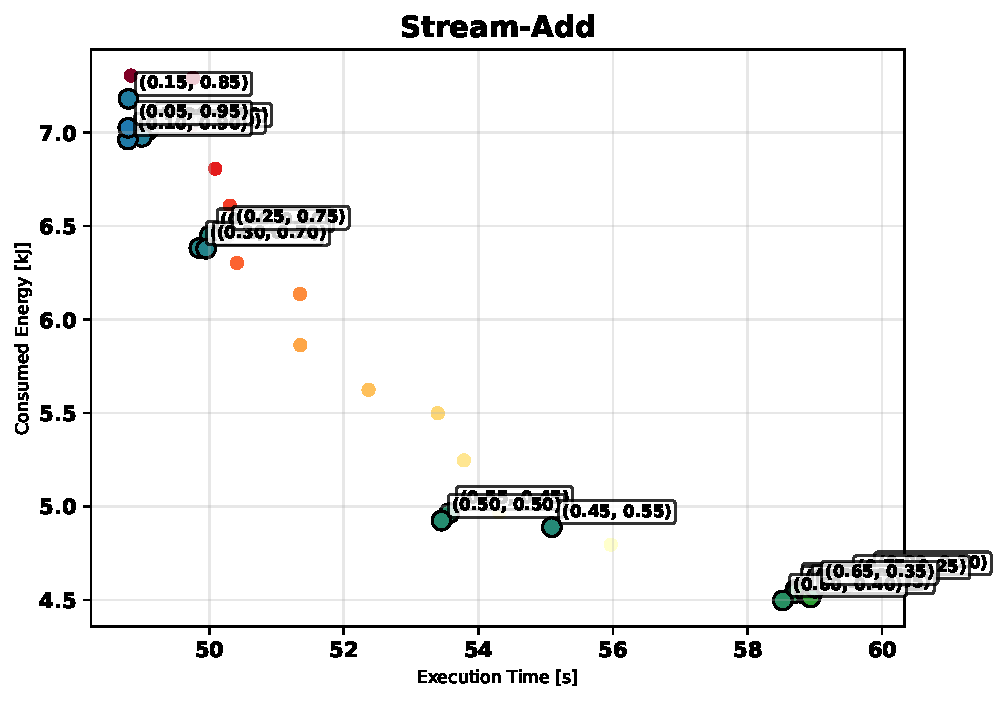
\includegraphics[width=\textwidth]{Figure/energy_vs_et/Energy_vs_time_ones-stream-add.pdf}
      \caption{Stream-Add}
      \label{fig:energy_time_add}
  \end{subfigure}
  \hfill
  \begin{subfigure}[b]{0.47\textwidth}
      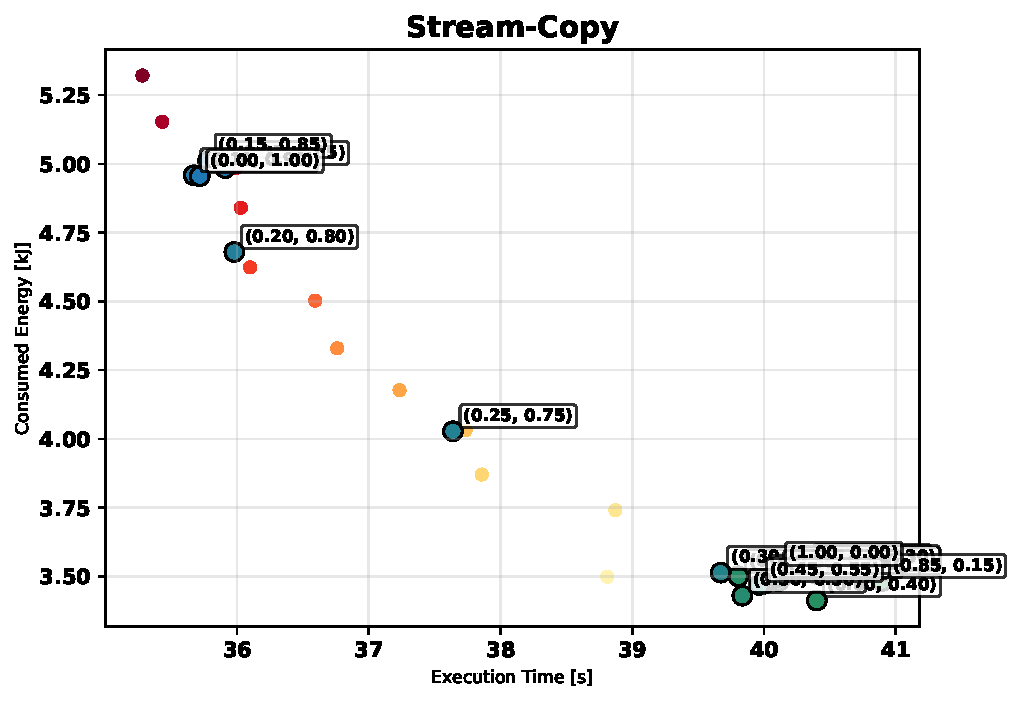
\includegraphics[width=\textwidth]{Figure/energy_vs_et/Energy_vs_time_ones-stream-copy.pdf}
      \caption{Stream-Copy}
      \label{fig:energy_time_copy}
  \end{subfigure}

  \vspace{0.5em}

  % Row 3 — centred
  \begin{subfigure}[b]{0.50\textwidth}
      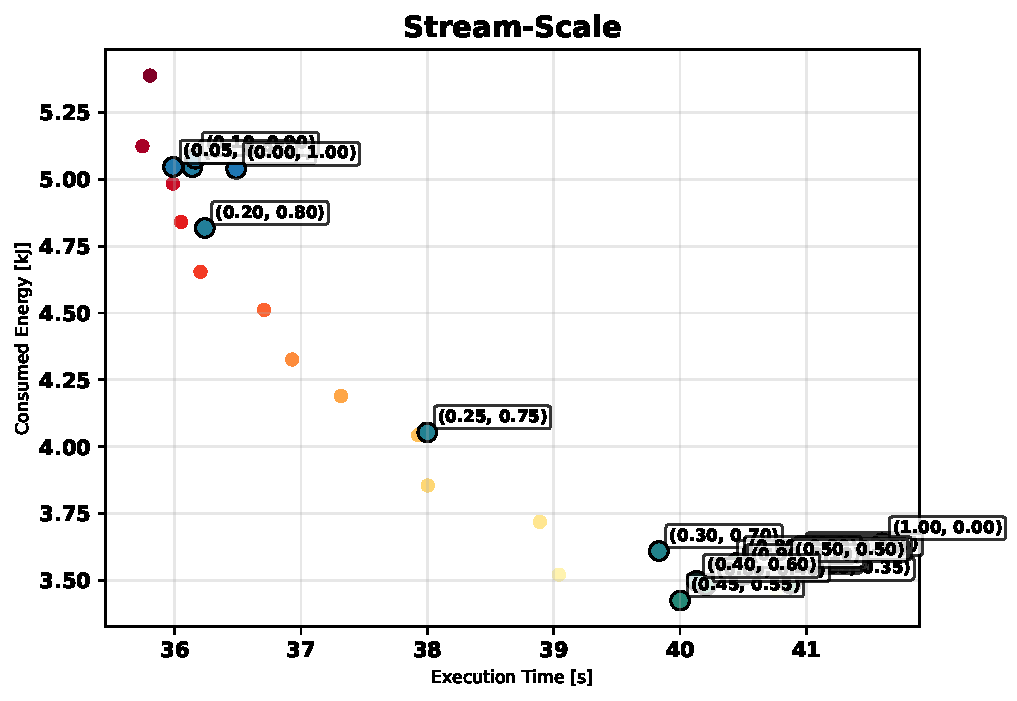
\includegraphics[width=\textwidth]{Figure/energy_vs_et/Energy_vs_time_ones-stream-scale.pdf}
      \caption{Stream-Scale}
      \label{fig:energy_time_scale}
  \end{subfigure}

  \caption{Execution time (s) vs.\ consumed energy (kJ) for the five
           STREAM memory-bandwidth benchmarks~\cite{stream} under DDMORL.
           Filled circles show DDMORL operating points under nine preference
           configurations; marker colour encodes the mean PCAP level (W)
           selected by the policy (colour bar, right).
           Open circles show static fixed-PCAP baselines~\cite{nrm} at each
           of the 14 discrete power cap levels.
           Across all five benchmarks, the RL policy consistently selects
           operating points on or near the lower-left convex hull of the
           static baseline scatter, confirming that the preference-conditioned
           policy learns to approximate the Pareto front rather than an
           arbitrary fixed cap.}
  \label{fig:energy_time_stream}
\end{figure*}

\noindent\textbf{Overlap with static baselines and absence of overhead.}
The central observation in Figures~\ref{fig:energy_time_stream} and~\ref{fig:energy_time_npb} is that each DDMORL filled circle falls on or in the immediate vicinity of the open-circle (static PCAP) point at the same execution time and energy coordinates. This spatial co-location has a direct operational interpretation: the RL controller arrives at precisely the same (energy, execution time) operating point that a statically configured power cap would produce, meaning no additional energy or runtime is spent on policy inference. Because Q-network evaluation occurs at PCAP control intervals (every $10$\,s) and involves only a single forward pass through a small network, its compute and energy footprint is negligible relative to the benchmark execution durations, which span tens of seconds to tens of minutes. The overlay therefore constitutes an empirical proof that DDMORL introduces no measurable overhead: running the adaptive controller is energetically equivalent to running the optimally tuned static power cap, while additionally providing the ability to tune the operating point through a single intuitive parameter $\delta$.

% ------------------------------------------------------------
% Figure 5.6 — Execution Time vs Energy: RL policy vs static PCAP (NPB)
% ------------------------------------------------------------
\begin{figure*}[tbp]
  \centering
  % Row 1
  \begin{subfigure}[b]{0.47\textwidth}
      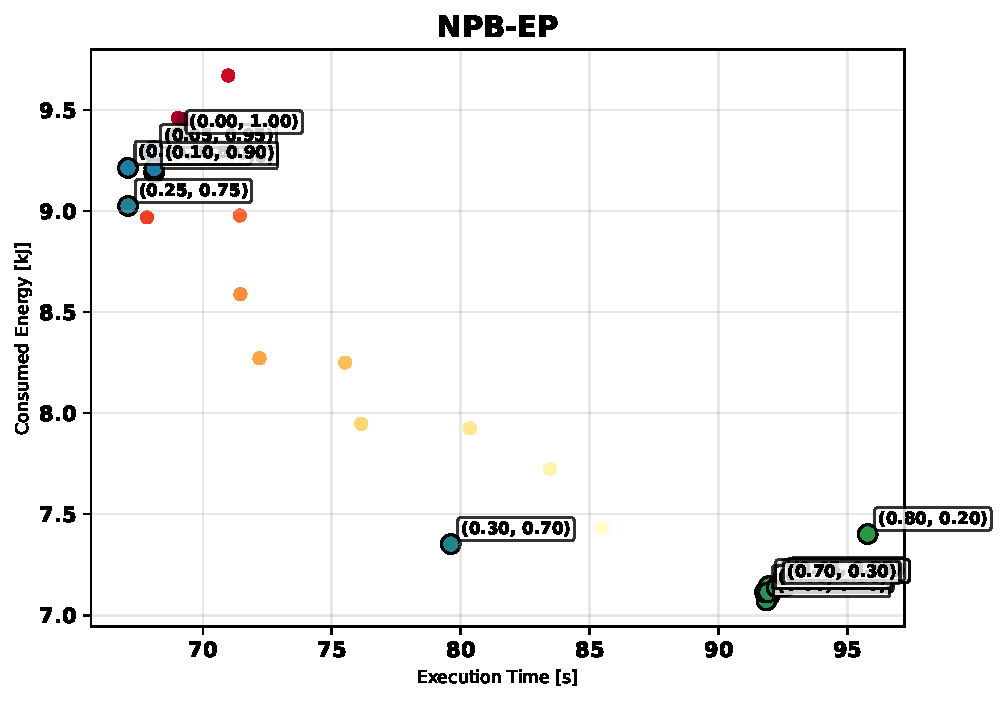
\includegraphics[width=\textwidth]{Figure/energy_vs_et/Energy_vs_time_ones-npb-ep.pdf}
      \caption{NPB-EP}
      \label{fig:energy_time_npb_ep}
  \end{subfigure}
  \hfill
  \begin{subfigure}[b]{0.47\textwidth}
      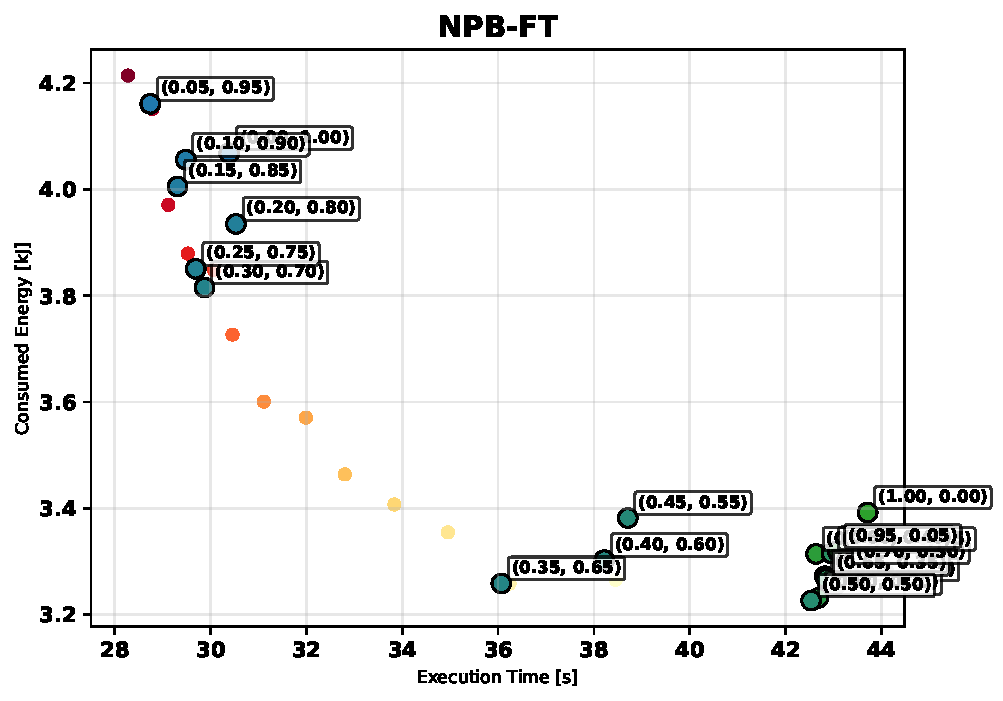
\includegraphics[width=\textwidth]{Figure/energy_vs_et/Energy_vs_time_ones-npb-ft.pdf}
      \caption{NPB-FT}
      \label{fig:energy_time_npb_ft}
  \end{subfigure}

  \vspace{0.5em}

  % Row 2
  \begin{subfigure}[b]{0.47\textwidth}
      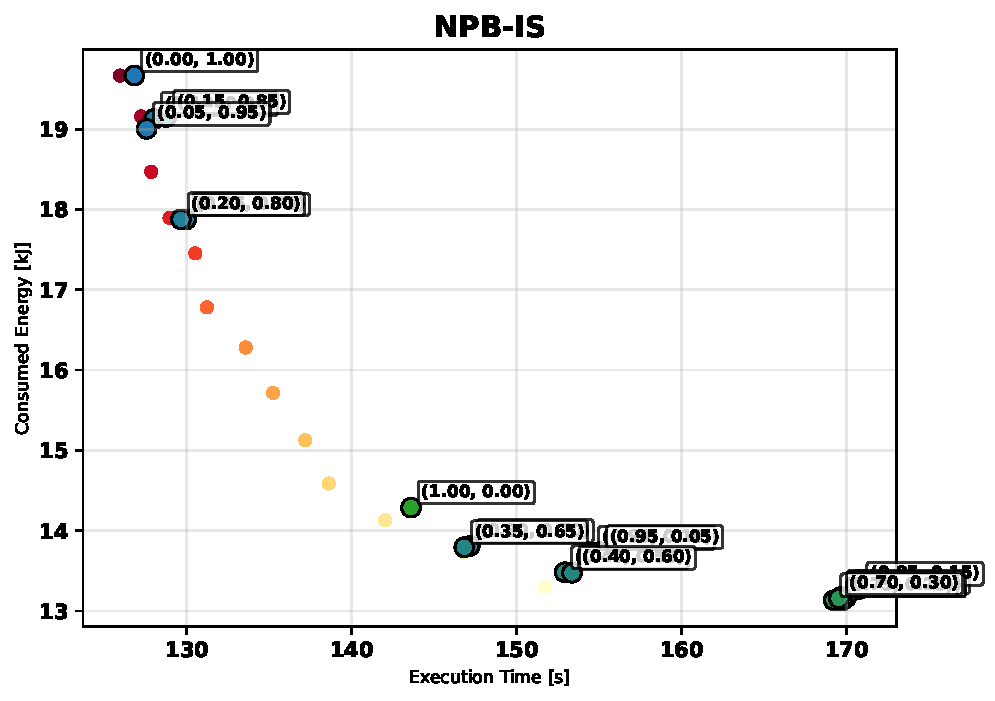
\includegraphics[width=\textwidth]{Figure/energy_vs_et/Energy_vs_time_ones-npb-is.pdf}
      \caption{NPB-IS}
      \label{fig:energy_time_npb_is}
  \end{subfigure}
  \hfill
  \begin{subfigure}[b]{0.47\textwidth}
      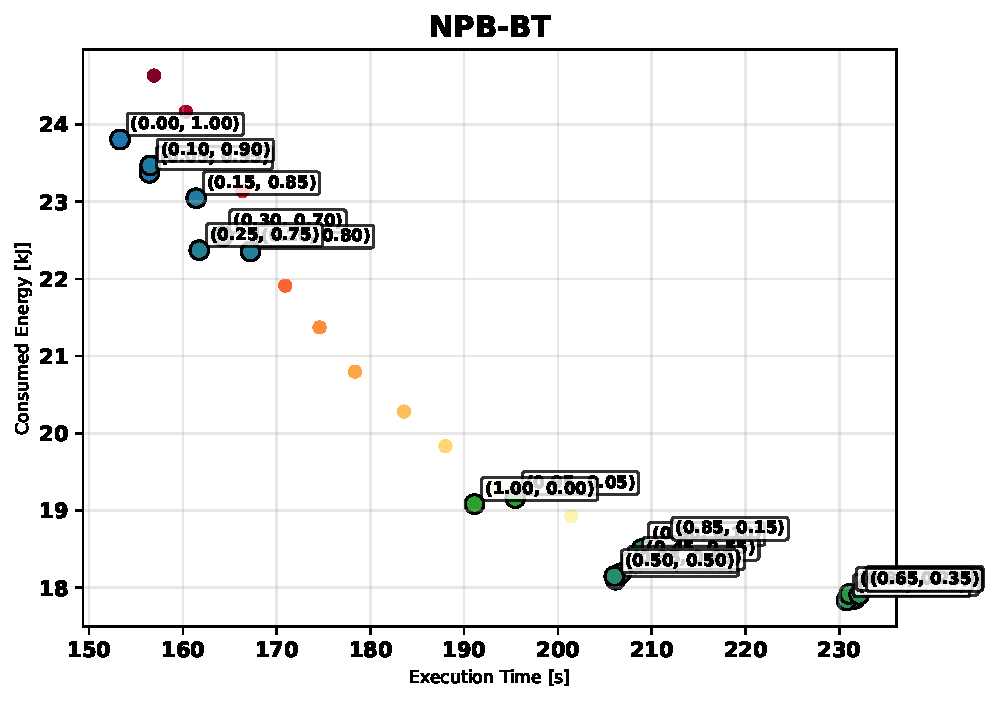
\includegraphics[width=\textwidth]{Figure/energy_vs_et/Energy_vs_time_ones-npb-bt.pdf}
      \caption{NPB-BT}
      \label{fig:energy_time_npb_bt}
  \end{subfigure}

  \caption{Execution time (s) vs.\ consumed energy (kJ) for the four
           NAS Parallel Benchmarks~\cite{npb} under DDMORL.
           Filled circles show DDMORL operating points under nine preference
           configurations; marker colour encodes the mean PCAP level (W)
           selected by the policy (colour bar, right).
           Open circles show static fixed-PCAP baselines~\cite{nrm} at each
           of the 14 discrete power cap levels.
           Trained on a mixed dataset of STREAM and NPB variants (NPB-FT held
           out), the policy selects operating points near the Pareto front of
           the static baseline scatter across all four NPB benchmarks, including
           the out-of-distribution NPB-FT workload.}
  \label{fig:energy_time_npb}
\end{figure*}

\noindent\textbf{Generalisation confirmed by the baseline overlay.}
For NPB benchmarks (Figure~\ref{fig:energy_time_npb}), the policy was trained on EP, IS, and BT variants but not on NPB-FT, which serves as the out-of-distribution test case. Across all four NPB benchmarks, filled-circle operating points track the convex hull of the static baseline scatter with fidelity comparable to STREAM. For NPB-IS and NPB-BT, operating points at $\delta \leq 0.3$ cluster near the high-PCAP ($\geq 130$\,W) open-circle group, while those at $\delta \geq 0.6$ align with the low-PCAP ($89$--$107$\,W) cluster. The consistent tracking across both in-distribution and out-of-distribution NPB workloads confirms that the PAPI-derived state features (IPC, L3 miss rate, and stall ratio) carry sufficient information for the controller to infer the appropriate power level without requiring separate per-workload training or PCAP profiling.
